\chapter{Etude terrain} % 40 pages

Lors de mon étude terrain, j'ai eu l'occasion de recenser l'avis de nombreuses personnes sur l'open source mais également sur les réflexions menée lors de mon état de l'art.

J'ai choisi d'orienter mes questionnaires et interview sur les 4 grands domaines qui représentent selon moi un pilier à améliorer, comprendre et faire évoluer pour valoriser l'open source et sur lesquel l'éditeur à la main.

Le questionnaire à été traité par 38 personnes, 89\% d'entre elles ont affirmés connaitre très bien l'open source 

	\section{Plateforme promotrice}

		\subsection{Une interface pour communiquer qui laisse à désirer}

			Autour des plateformes qui contiennent et promouvoie l'open source, sur 31 personnes enregistrées pour cette question, 20 indiquent qu'il y a un manque à palier dans l'interface qui permet de communiquer avec l'éditeur open source. 

			\begin{figure}[h]
				\center
				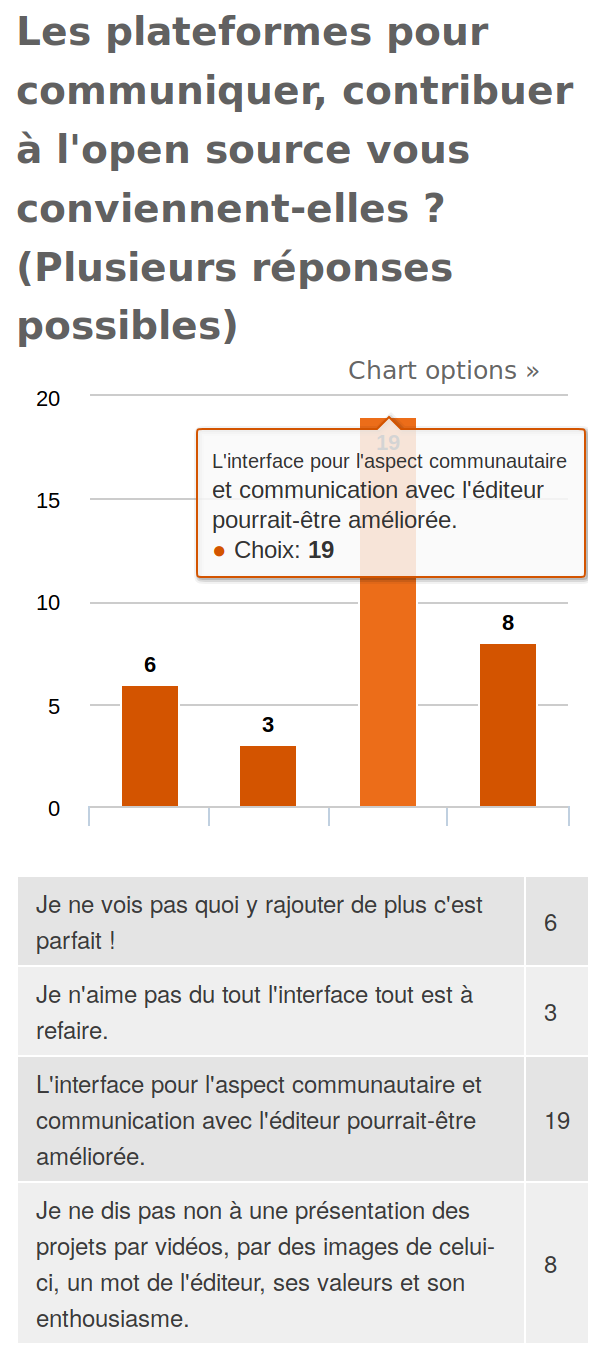
\includegraphics[scale=0.28]{./img/a9}
				\caption{Communication avec l'éditeur}
			\end{figure}

			\newpage

			Lors de l'interview auprès de Olivier Magnial, ingénieur systèmes embarqués chez l'une des plus grande entreprise promotrice de l'open source : SMILE. Celui-ci à déclaré : 

			\begin{center}
				\textit{
				\textquote{
					Pour \gls{mainliner} du code source, un processus décrit la manière de contribuer, et c'est le plus souvent par mail.(...) Linux, par exemple c'est entièrement du mail, on à des mailing list extrêmement longues et des processus assez carrés !
				}
				}
			\end{center}

		\subsection{Un module de présentation}

			Sur la question:

			\begin{center}
				\textit{
				\textquote{
					Les plateformes pour communiquer, contribuer à l'open source vous conviennent-elles ?
				}
				}
			\end{center}

			Seulement 8 personnes sur 31 personnes qui ont répondu à celle-ci sont intéressé pour avoir une présentation sous forme de vidéo du projet, avec un mot de l'éditeur qui communique ses ambitions, ses valeurs.

			\begin{figure}[h]
				\center
				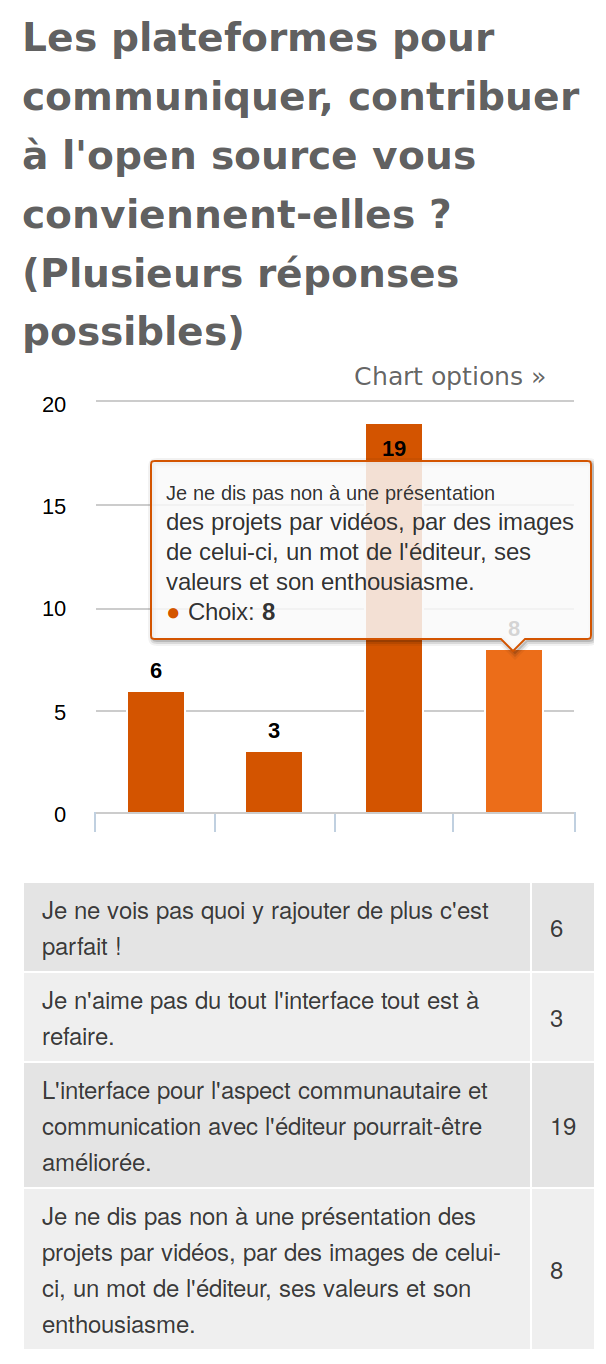
\includegraphics[scale=0.28]{./img/a92}
				\caption{Module de présentation}
			\end{figure}

			Lors de l'interview de Quentin Cazelles, Ingénieur développeur chez Docdoku, celui-ci mentionne tout de même le fait qu'une vitrine à ces plateformes s'impose pour les consommateurs finaux qui ne sont pas développeur.

			\begin{center}
				\textit{
				\textquote{
					La plateforme est un frein pour l'utilisateur final non développeur, il faudrait en effet mettre une vitrine dans un style plus commercial (...)
				}
				}
			\end{center}

			\newpage

		\subsection{Pas d'extrèmes sur les plateformes}

			Très peu de contributeur, c'est-à-dire 6 sur 30, répondent que les plateformes sont parfaites et qu'il ne vois pas d'amélioration potentielles.

			Il n'y a pas non plus beaucoup d'insatisfait sur celles-ci car seulement 3 ont répondu que toute l'interface était à refaire.

	\section{Gestion des ressources}

	\newpage
	\section{Chez le consommateur}

		\subsection{La contribution du consommateur}

		Dans les personnes interrogés, beaucoup souhaite contribuer ou ont déjà contribué à l'open sources ou souhaitent le faire un jour prochain.60\% y ont déjà contribué, 28\% souhaitent y contribuer un jour.

		\begin{figure}[h]
			\center
			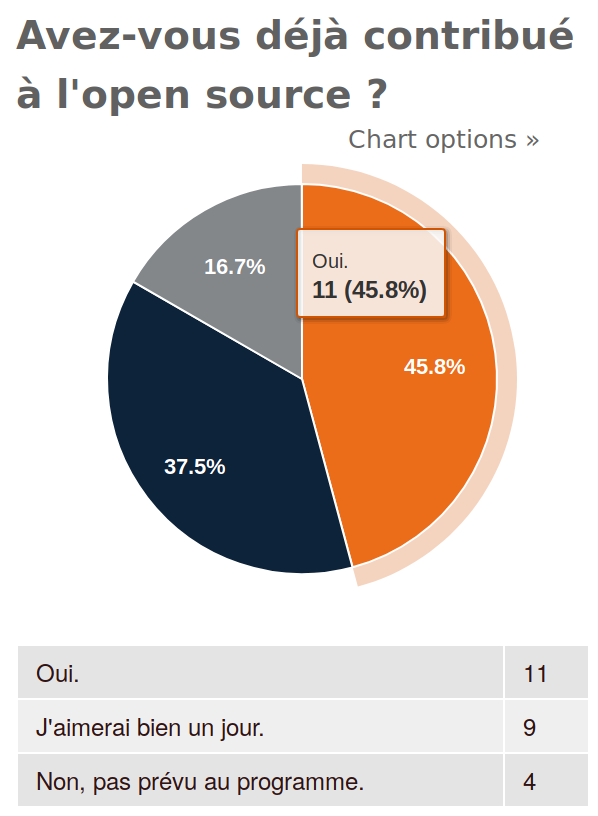
\includegraphics[scale=0.58]{./img/a4}
			\caption{Contribution à l'open source}
		\end{figure}

		\newpage

		Et ce quelque soit leur domaines d'activité. Sur les 37 personnes recensées, les domaines d'activités, même si une majoritée est dans l'informatique, sont divers:

		\begin{itemize}[label=\textbullet, font=\LARGE \color{burntorange}]
			\item Edition, Communication, Multimédia
			\item Etude et conseils
			\item Informatique / Télécom
			\item Industriel
			\item Autres
		\end{itemize}

		\begin{figure}[h]
			\center
			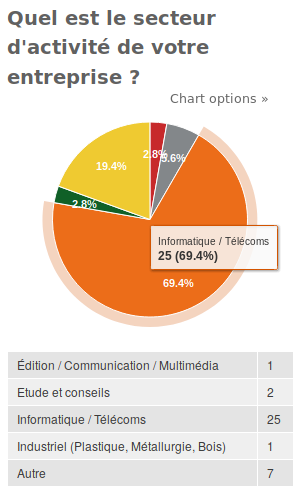
\includegraphics[scale=0.58]{./img/a1}
			\caption{Secteur d'activité des personnes interrogées}
		\end{figure}

		\newpage

		\subsection{Le ressenti du consommateur à contribuer}

		J'ai posé une question dans mon questionnaire autour de la perçeption que les gens peuvent avoir dans l'accueil de contribution, s'ils avait des peur ou au contraire qu'il est très agréable de partager avec l'editeur et la communauté ses contributions.

		Globalement, aucun frein n'est ressenti à la contribution et son accueil par l'éditeur, même si ces personnes ne contribuent par pour autant:

		\begin{itemize}[label=\textbullet, font=\LARGE \color{burntorange}]
			\item 46\% des interrogés ont répondu que leurs contribution était très bien accueilli, que l'éditeur et la communauté était agréable.
			\item 43\% Ne prennent pas le temps de contribuer mais n'y vois aucun blocage.
			\item Et seulement 11\% ont peur de contribuer et d'être jugé.
		\end{itemize}

		Dans leur entreprise, ces personnes considèrent pourtant majoritairement que l'open source est essentiel ou nécessaire.

		Pour 10 personnes, l'open source est essentiel et ils y attachent beaucoup d'importance.
		12 questionnés disent que l'open source est nécessaire dans leur projets. 8 personnes disent qu'ils ne s'en soucient pas vraiment dans leur entreprise et 5 personne n'ont jamais entendu parlé d'open source dans leur société.

		\begin{figure}[h]
			\center
			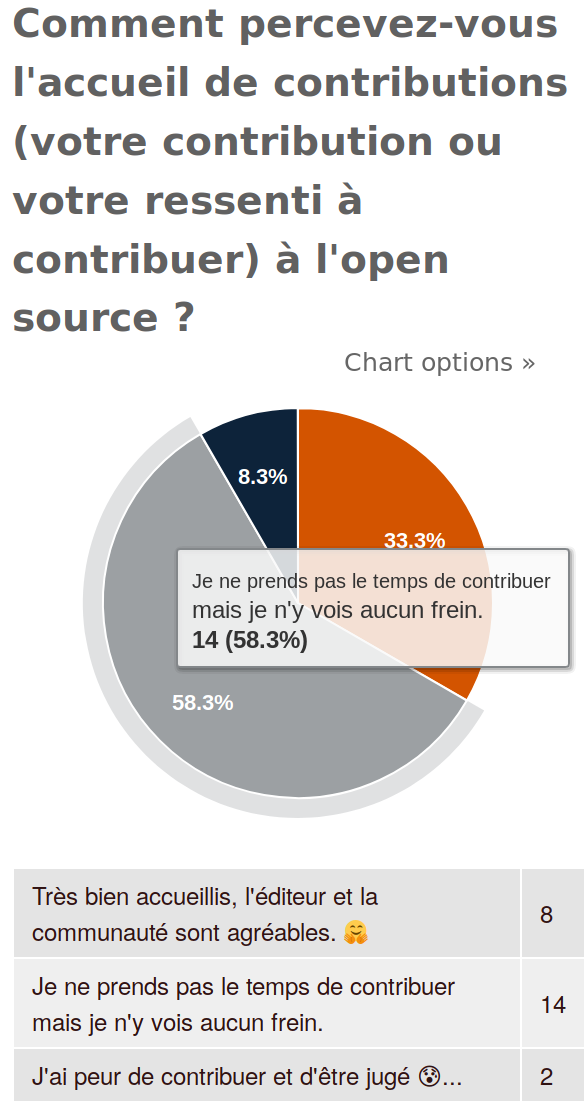
\includegraphics[scale=0.58]{./img/a7}
			\caption{Perception de contribution à l'open source}					
		\end{figure}

		\newpage

		\subsection{Le support payant}

		Dans l'ensemble des personnes interrogés, une forte majorité indiquent qu'ils ne sont pas contre payer du support pour un logiciel open source. 12 personnes ont répondu qu'il était nécessaire et abordable en général. 22 personnes n'ont pas d'objection à payer pour du support logiciel et comprennent qu'il faille rémunérer l'éditeur d'une certaine façon. Et seulement 3 ont répondu qu'il pensait que l'open source devait être gratuit

		\begin{figure}[h]
			\center
			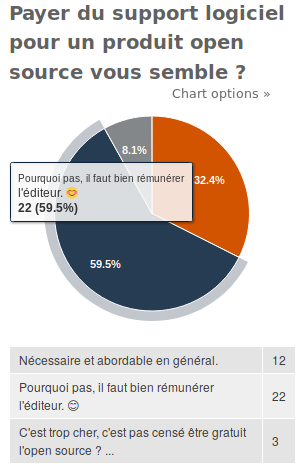
\includegraphics[scale=0.58]{./img/a11}
			\caption{Payer du support logiciel}					
		\end{figure}

	\newpage

	\section{Marketing de l'open source}

		\subsection{L'école et l'open source}

			Sur une 30aine de personnes qui ont répondu à la question: "Devrait on sensibiliser les gens à l'open source dans les écoles informatiques ?", je constate que 12 de ces personnes ont découvert l'open source par le biais de l'école.

			\begin{figure}[h]
				\center
				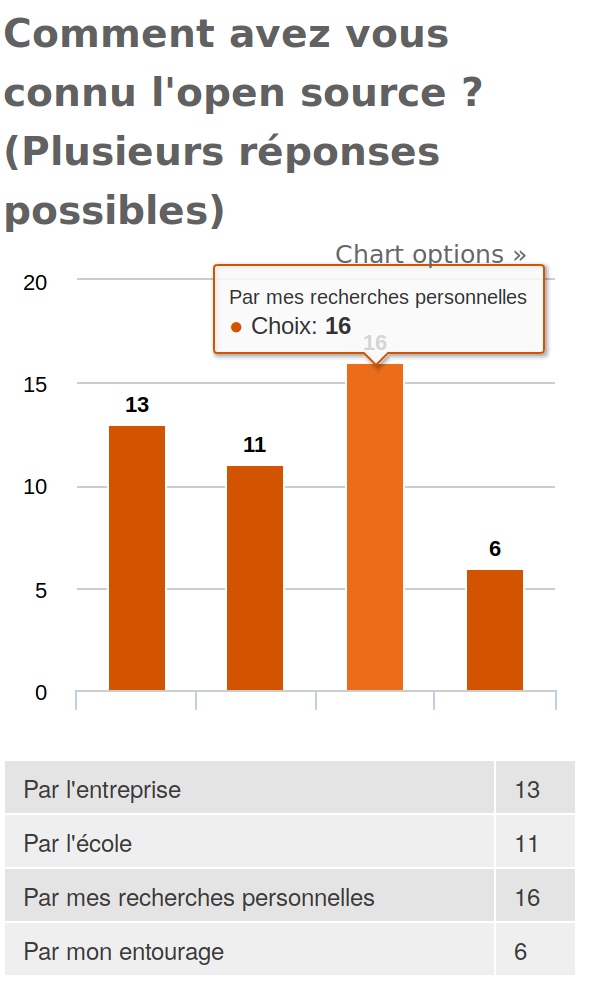
\includegraphics[scale=0.28]{./img/a3}
				\caption{Découverte de l'open source}
			\end{figure}

			\newpage

			Une majoritée des contributeurs, soit 92\% mentionne que l'on devrait bel et bien sensibiliser les gens à l'open source dans les écoles informatiques

			Seulement 3 personnes, dont 2 qui ont découvert l'open source à l'école, trouvent que c'est déjà fait intrinsèquement au programme.

			\begin{figure}[h]
				\center
				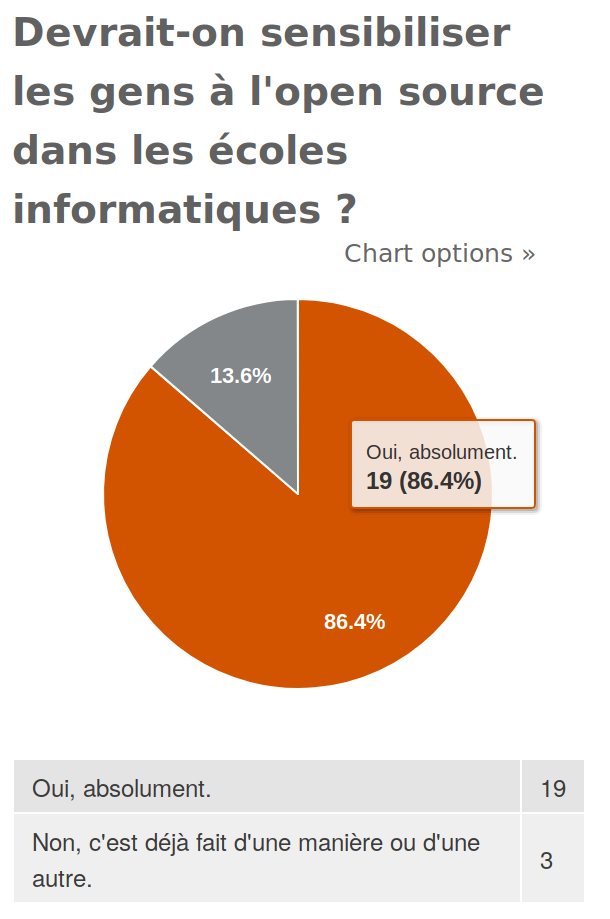
\includegraphics[scale=0.28]{./img/a6}
				\caption{Sensibiliser à l'open source}
			\end{figure}

			\newpage

			Plus de la moitiée de ces personnes, soit 21 interrogé ont répondus que l'open source était peu ou tout juste assez évoqué à l'école.

			9 personnes trouvent que les écoles informatique traitent suffisamment de l'open souce

			Seulement 1 personne à déclaré que l'open source était fortement présent dans les écoles informatiques

			\begin{figure}[h]
				\center
				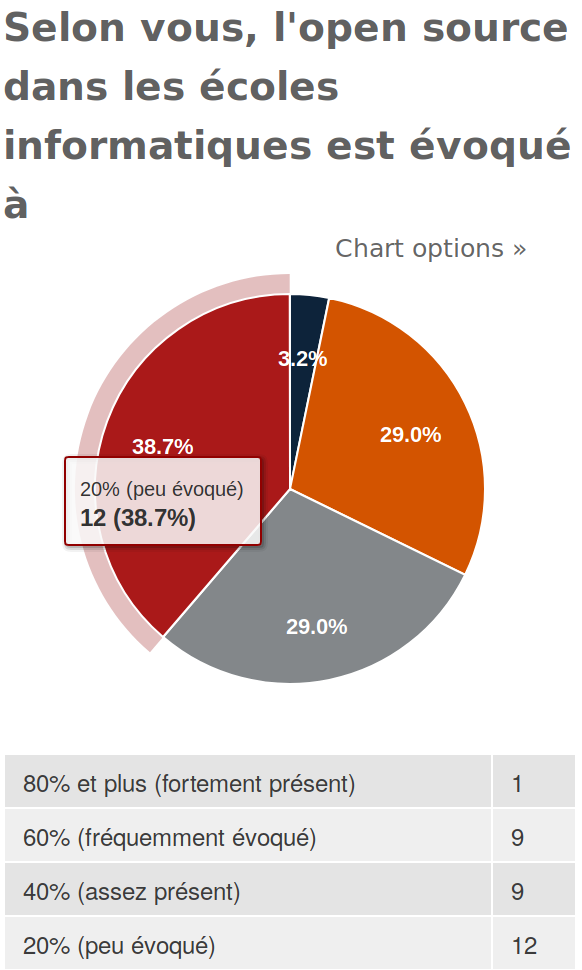
\includegraphics[scale=0.28]{./img/a5}
				\caption{L'open source à l'école}					
			\end{figure}









